\chapter{Problems}
There are several problems with the design that limit the usability
and the ability of the design to reach its design goals.
In this chapter we will explain the problems and their impact.

\section{Branch attack}
In this section we will explain an attack that can be done by a malicious node M.

\subsection{Abandoning full transaction history distribution}
One of the main pillars of the design is to not distribute
and have one common, full transaction history(TH) between every peer.
While this is the main pillar of design for the blockchain of Bitcoins.
The reasoning behind the idea to abandon is that a common, full truth
will the amount of interactions in scalability or the participiation of less powerfull machines.

The reason for the limitation is that every interactions will have to be distributed to every peer in the network.
This will come at the cost of bandwidth, compute power and storage for every node for every transaction.
The cost might be very limited for a single transaction,
but with greater scale these cost will add up.
The amount of these three resources is limited and will limit the amount of transactions that can be processed.

The limitation can be delayed by excluding particitpation of lesser powerfull devices.
For example, mobile devices have generally much less storage available.
When the full TH becomes too large,
participation of these mobile devices is excluded due to the fact that they cannot fully store the TH.
This problem can be seen to affect Bitcoins and has been demonstrated in section \ref{bitcoin-limit-size}.
Mobile devices now typically operate in the less secure SPV mode.

\subsection{Alternating partial transaction history}
A malicious node M has his own chain of transactions
and he might not be happy with his transactions starting from a certain point.
He wants to rewrite history from that point and create an alternate TH.
The node can simply choose to forget and obscure blocks after that point.
A new branch will be created by chaining new blocks to the desired point in history.

\begin{figure}
	\centerline{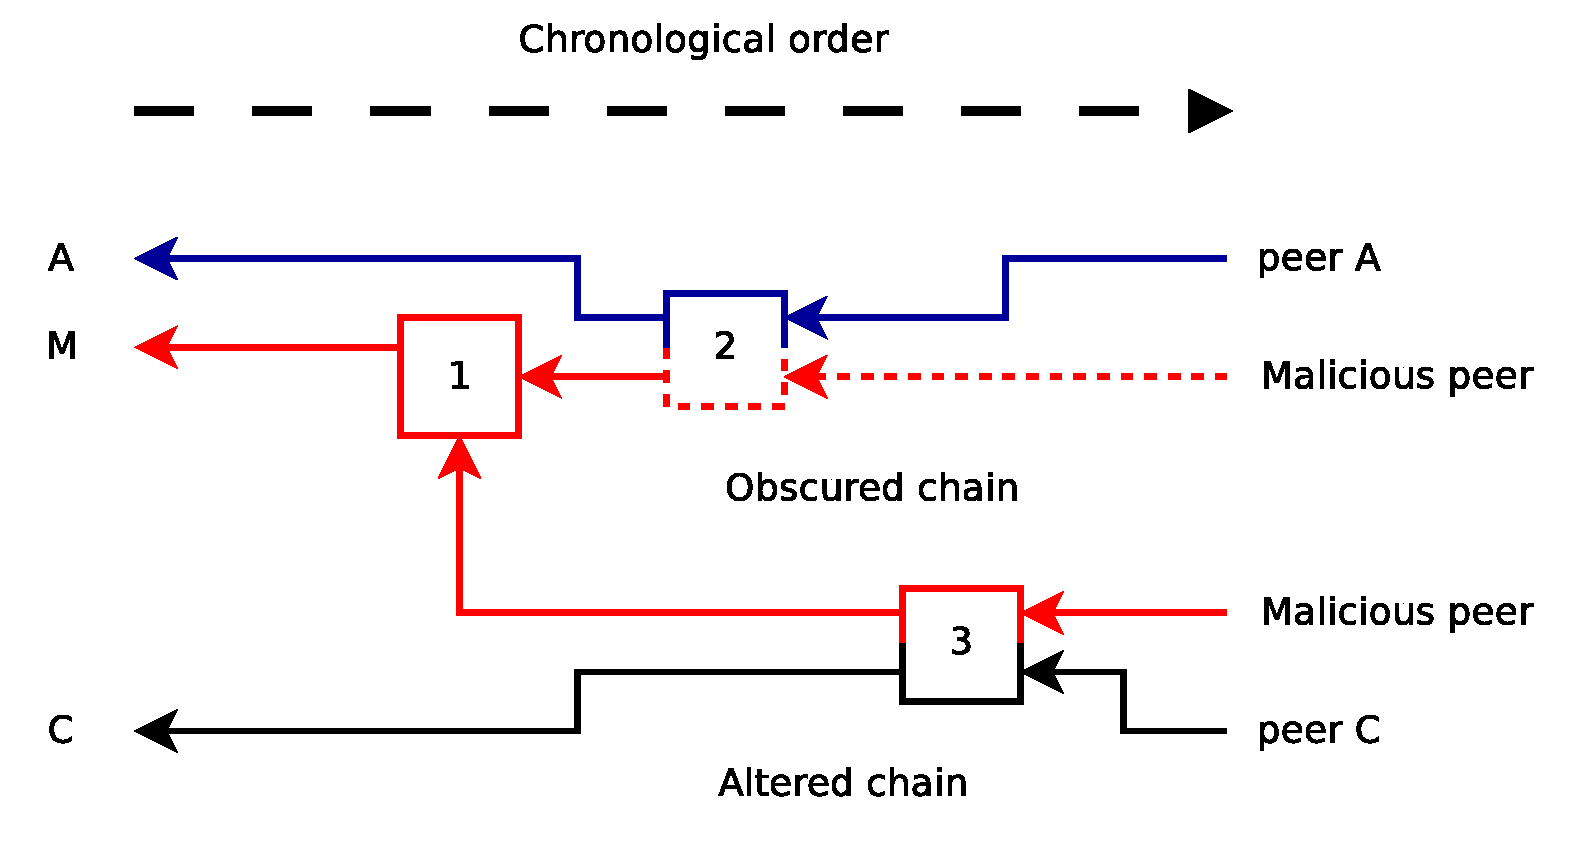
\includegraphics[scale=0.3]{problems/figs/branch.eps}}
	\caption{Example of a branch created by M.}
	\label{fig:problem-branch-obscure}
\end{figure}

In Figure \ref{fig:problem-branch-obscure} an example can be seen of a branch created by M.
In this example M tries to obscure block 2 and any subsequent blocks from C.
When C requests the TH of M, M will only send the TH up to block 1.
If M and C create a block together,
then M will reuse the hash of block 1 in the new block.
For clarity of the diagram, the node interacting with M in block 1 is not displayed.

Now malicious node M does have the problem that not only he knows his TH.
When node M interacted with node A a block was created that node M tries to obscure.
A has this block in his own chain
and therefore knows about it being part of the TH of M.
This can be seen in the example in Figure \ref{fig:problem-branch-obscure}.

M will want to reduce the likelyhood of the detection of his fraud.
If his fraud is detected, he might be punished and no longer to continue his abuse.
The first way to minimize detection is to choose
to only interact with new nodes that do not know about the alternate part of the TH.
Nodes that have requested an alternate part of the TH
or that have been interacted directly with are no longer interacted with.
In a sufficiently healthy network this will result in node M being able to find new nodes to help him.

\begin{figure}
	\centerline{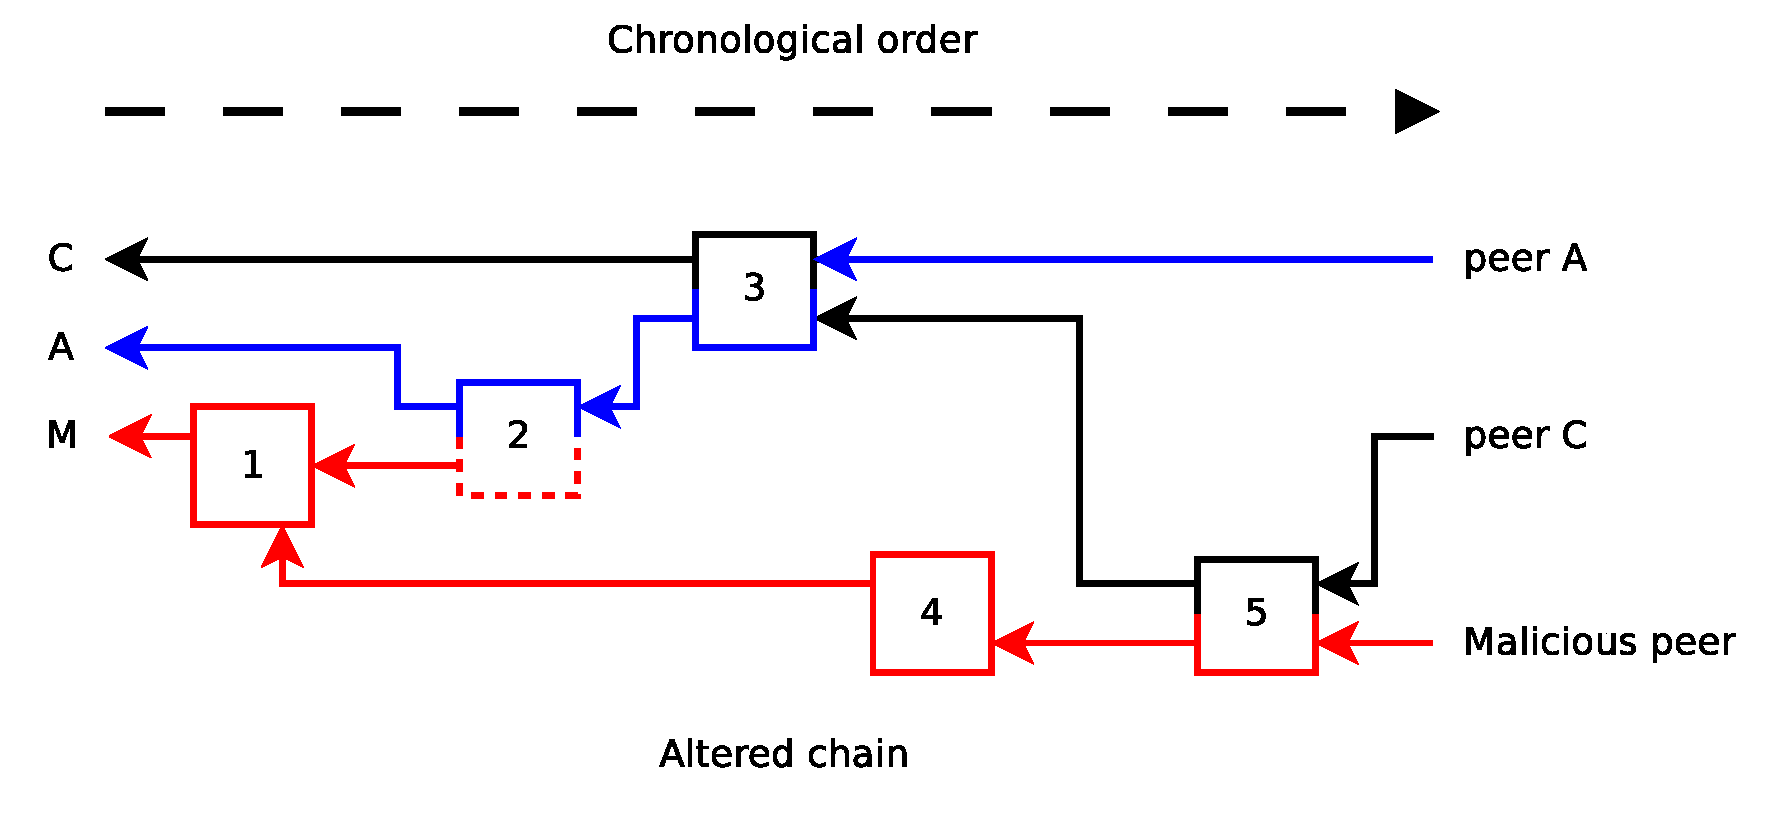
\includegraphics[scale=0.3]{problems/figs/branch-fraud-detected.eps}}
	\caption{Detectable fraud by C.}
	\label{fig:problem-branch-preknowledge}
\end{figure}

There is another example that will expose the fraud of M.
This example can be seen in Figure \ref{fig:problem-branch-preknowledge}.
A node C might still exposes the cheating of M by chance.
C can have an interaction with node A by coincidence.
Before creating block 3 C will request the TH of node A containing an obscured block of M.
Now when M wants to interact with C, M will want to create block 5.
When C requests the full TH of M, it will detect that the TH of M no longer contains block 2.
This exposes the fraud of M.

But C will have no sure way of exposing this type of fraud by his own doing,
except for requesting every TH of every node in the system.
This is in a way a common, full TH and was chosen to be avoided by the design to become more scalable.
C can limited the possibility of the attack by increasing his knowledge by collecting more TH of other nodes.
If node A or B stop participating and exit,
then C will have no way of detecting the fraud by M.

The second way M can limit the exposure of his cheating is in a more sophisticated way.
He can present several, different TH to different nodes.
M will continue keeping track of the unmodified TH.
When M wants to interact with A or B, both knowing this TH, he will present this TH.
So M can still interact with A and B.
But when interacting with C he will present his alternate TH.
C will only expose the fraud in the same way as previously.

\subsection{Possibility of attack and likelyhood of detecting fraud}
This attack can always be done M and is not limited to circumstances.
The likelyhood of exposing this attack depends on several factors
and will be the only factor to limit M in performing this fraud.
The likelihood depends on:
\begin{itemize}
\item Size of the network
\item Likelihood of interactions between A or B and C
\end{itemize}

All these properties will influence the chance of C coming across an obscured block.

\subsection{Possible punishment of this attack}
When the fraud is detected C can only punish M by no longer interacting with him.
There is currently no way of making it globally know to every node in the network that fraud was committed.
So only M is punished by C and can continue his abuse of other nodes in the network.


